\documentclass[a4paper, 12pt]{article}

\usepackage[utf8]{inputenc}
\usepackage{amsmath}

\usepackage[]{amsfonts}
\usepackage[]{graphicx}

\title{CS231A Course Notes 5: Active and Volumetric Stereo}
\author{Kenji Hata and Silvio Savarese}
\date{}

\renewcommand\emph{\textbf}

\numberwithin{equation}{section}
\begin{document}

\maketitle

\section{Introduction}
In traditional stereo, the main idea is to use corresponding points $p$ and $p'$ to estimate the location of a 3D point $P$ by triangulation. A key challenge here, is to solve the correspondence problem: how do we know whether a point $p$ actually corresponds to a point $p'$ in another image? This problem is further accentuated by the fact that we need to handle the many 3D points that are present in the scene. The focus of these notes will discuss alternative techniques that work well in reconstructing the 3D structure.

\section{Active stereo}
\begin{figure}[h!]
    \centering
    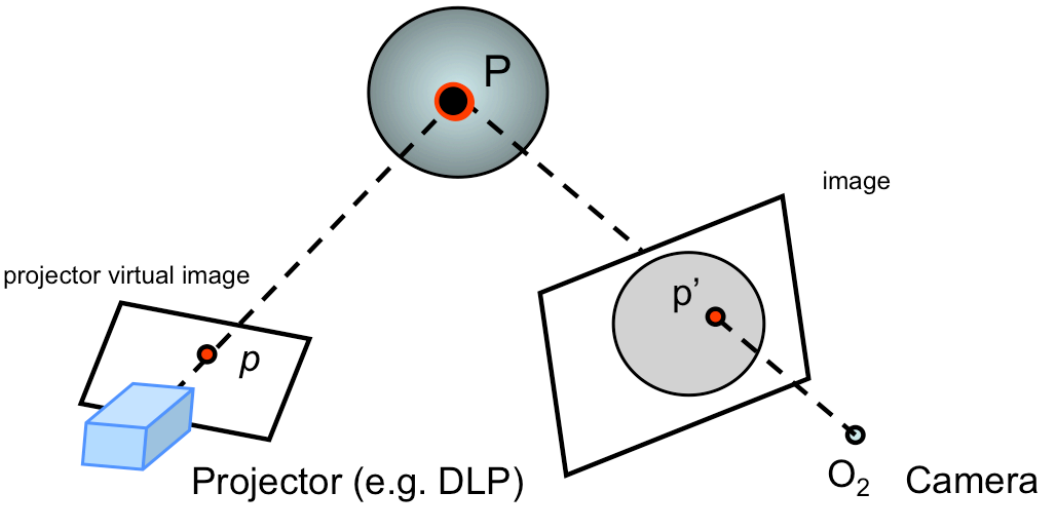
\includegraphics[width = 0.8\textwidth]{figures/active_stereo_setup.png}
    \caption{The active stereo setup that projects a point into 3D space.}
    \label{fig:active_stereo_setup}
\end{figure}

First, we will an introduce a technique known as \emph{active stereo} that helps mitigate the correspondence problem in traditional stereo. The main idea of active stereo is to replace one of the two cameras with a device that interacts with the 3D environment, usually by projecting a pattern onto the object that is easily identifiable from the second camera.  This new projector-camera pair defines the same epipolar geometry that we introduced for camera pairs, whereby the image plane of the replaced camera is replaced with a \emph{projector virtual plane}. In Figure~\ref{fig:active_stereo_setup}, the projector is used to project a point $p$ in the virtual plane onto the object in 3D space, producing a point in 3D space $P$. This 3D point $P$ should be observed in the second camera as a point $p'$. Because we know what we are projecting (e.g. the position of $p$ in the virtual plane, the color and intensity of the projection, etc.), we can easily discover the corresponding observation in the second camera $p'$. 

\begin{figure}[h!]
    \centering
    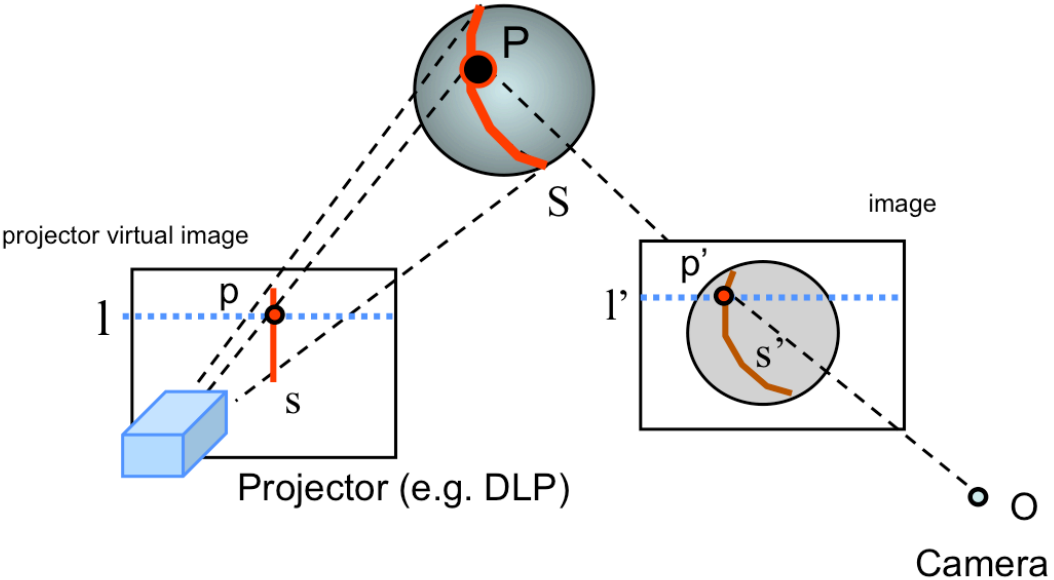
\includegraphics[width = 0.8\textwidth]{figures/active_stereo_line.png}
    \caption{The active stereo setup that projects a line into 3D space.}
    \label{fig:active_stereo_line}
\end{figure}

A common strategy in active stereo is to project from the virtual plane a vertical stripe $s$ instead of a single point. This case is very similar to the point case, where the line $s$ is projected to a stripe in 3D space $S$ and observed as a line in the camera as $s'$. If the projector and camera are parallel or rectified, then we can discover the corresponding points easily by simply intersecting $s'$ with the horizontal epipolar lines. From the correspondences, we can use the triangulation methods introduced in the previous course notes to reconstruct all the 3D points on the stripe $S$. By swiping the line across the scene and repeating the process, we can recover the entire shape of all visible objects in the scene. 

Notice that one requirement for this algorithm to work is that the projector and the camera need to be calibrated. An active stereo system can be calibrated using similar techniques as described in previous notes. We can first calibrate the camera using a calibration rig. Then, by projecting known stripes onto the calibration rig, and using the corresponding observations in the newly calibrated camera, we can set up constraints for estimating the projector intrinsic and extrinsic parameters. Once calibrated, this active stereo setup can produce very accurate results. In 2000, Marc Levoy and his students at Stanford demonstrated that by using a finely tuned laser scanner, they could recover the shape of Michaelangelo's Pieta with sub-millimeter accuracy.

However, in some cases, having a finely tuned projector may be too expensive or cumbersome. An alternative approach that uses a much cheaper setup leverages shadows to produce active patterns to the object we want to recover. By placing a stick between the object and a light source at a known position, we can effectively project a stripe onto the object as before. Moving the stick allows us to project different shadow stripes onto the object and recover the object in a similar manner as before. This method, although much cheaper, tends to produce less accurate results because it requires very good calibration between the stick, camera, and light source, while needing to maintain a tradeoff between the length and thinness of the stick's shadow.

\begin{figure}[h!]
    \centering
    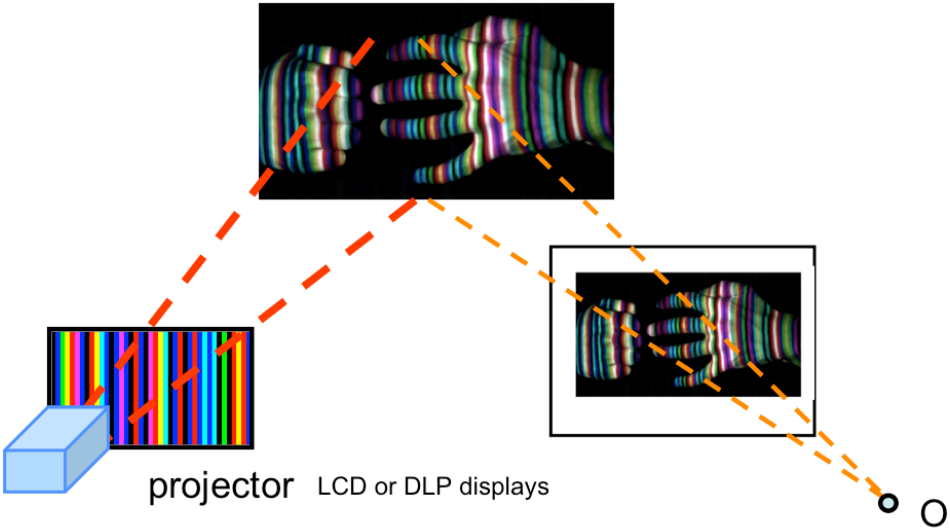
\includegraphics[width = 0.8\textwidth]{figures/active_multicolor_setup.png}
    \caption{The active stereo setup that uses multiple colored lines to reconstruct an object from a single projection.}
    \label{fig:active_multicolor_setup}
\end{figure}

One limitation of projecting a single stripe onto objects is that it is rather slow, as the projector needs to swipe across the entire object. Furthermore, this means that this method cannot capture deformations in real time. A natural extension is to instead attempt to reconstruct the object from projecting a single frame or image. The idea is to project a known pattern of different stripes to the entire visible of the object, instead of a single stripe. The colors of these stripes are designed in such a way that the stripes can be uniquely identified from the image. Figure~\ref{fig:active_multicolor_setup} illustrates this multiple color-coded stripes method. This concept powered many versions of modern depth sensors, such as the original version of the Microsoft Kinect. In practice, these sensors use infrared laser projectors , which  allow it to capture video data in 3D under any ambient light conditions. 

\section{Volumetric stereo}
\begin{figure}[h!]
    \centering
    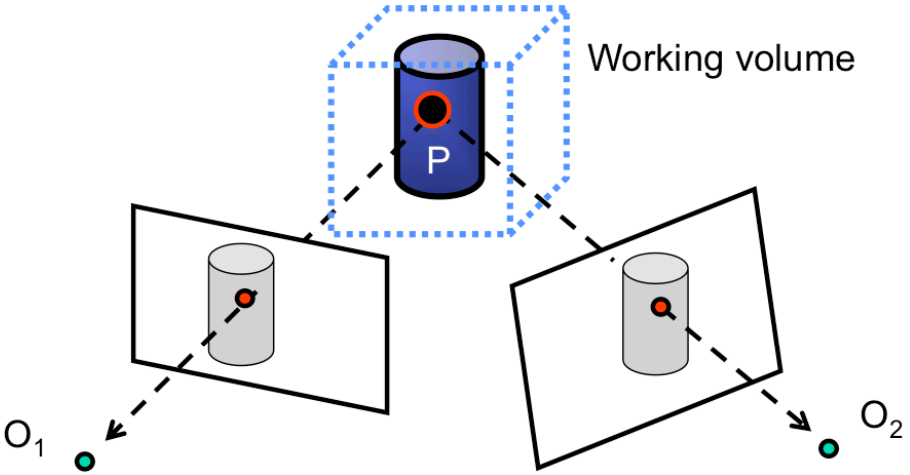
\includegraphics[width = 0.8\textwidth]{figures/volumetric_setup.png}
    \caption{The setup of volumetric stereo, which takes points from a limited, working volume and performs consistency checks to determine 3D shape.}
    \label{fig:volumetric_setup}
\end{figure}
An alternative to both the traditional stereo and active stereo approach is \emph{volumetric stereo}, which inverts the problem of using correspondences to find 3D structure. In volumetric stereo, we assume that the 3D point we are trying to estimate is within some contained, known volume. We then project the hypothesized 3D point back into the calibrated cameras and validate whether these projections are consistent across the multiple views. Figure~\ref{fig:volumetric_setup} illustrates the general setup of the volumetric stereo problem. Because these techniques assume that the points we want to reconstruct are contained by a limited volume, these techniques are mostly used for recovering the 3D models of specific objects as opposed to recovering models of a scene, which may be unbounded. 

The main tenet of any volumetric stereo method is to first define what it means to be ``consistent'' when we reproject a 3D point in the contained volume back into the multiple image views. Thus, depending on the definition of the concept of consistent observations, different techniques can be introduced. In these notes, we will briefly outline three major techniques, which are known as space carving, shadow carving, and voxel coloring.

\subsection{Space carving}
\begin{figure}[h!]
    \centering
    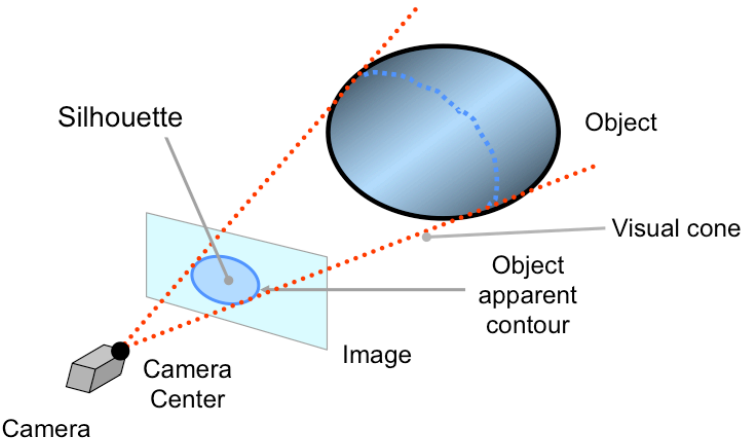
\includegraphics[width = 0.8\textwidth]{figures/visual_cone.png}
    \caption{The silhouette of an object we want to reconstruct contains all pixels of the visible portion of the object in the image. The visual cone is the set of all possible points that can project into the silhouette of the object in the image.}
    \label{fig:visual_cone}
\end{figure}
The idea of space carving is mainly derived from the observation that the contours of an object provide a rich source of geometric information about the object. In the context of multiple views, let us first set up the problem illustrated in Figure~\ref{fig:visual_cone}. Each camera observes some visible portion of an object, from which a contour can be determined. When projected into the image plane, this contour encloses a set of pixels known as the \emph{silhouette} of the object in the image plane. Space carving ultimately uses the silhouettes of objects from multiple views to enforce consistency.

However, if we do not have the information of the 3D object and only images, then how can we obtain silhouette information? Luckily, one practical advantage of working with silhouettes is that they can be easily detected in images if we have control of the background behind the object that we want to reconstruct. For example, we can use a ``green screen" behind the object to easily segment the object from its background.

Now that we have the silhouettes, how can we actually use them? Recall that in volumetric stereo, we have an estimate of some volume that we guarantee that the object can reside within. We now introduce the concept of a \emph{visual cone}, which is the enveloping surface defined by the camera center and the object contour in the image plane. By construction, it is guaranteed that the object will lie completely in both the initial volume and the visual cone. 

\begin{figure}[h!]
    \centering
    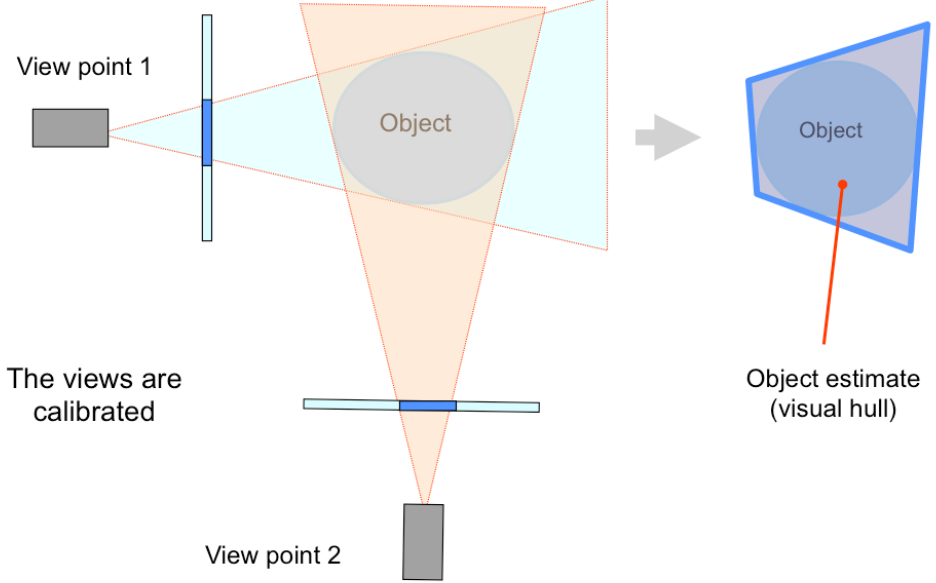
\includegraphics[width = 0.8\textwidth]{figures/visual_hull.png}
    \caption{The process of estimating the object from multiple views involves recovering the visual hull, which is the intersection of visual cones from each camera.}
    \label{fig:visual_hull}
\end{figure}

Therefore, if we have multiple views, then we can compute visual cones for each view. Since, by definition, the object resides in each of these visual cones, then it must lie in the intersection of these visual cones, as illustrated in Figure~\ref{fig:visual_hull}. Such an intersection is often called a \emph{visual hull}. 

\begin{figure}[h!]
    \centering
    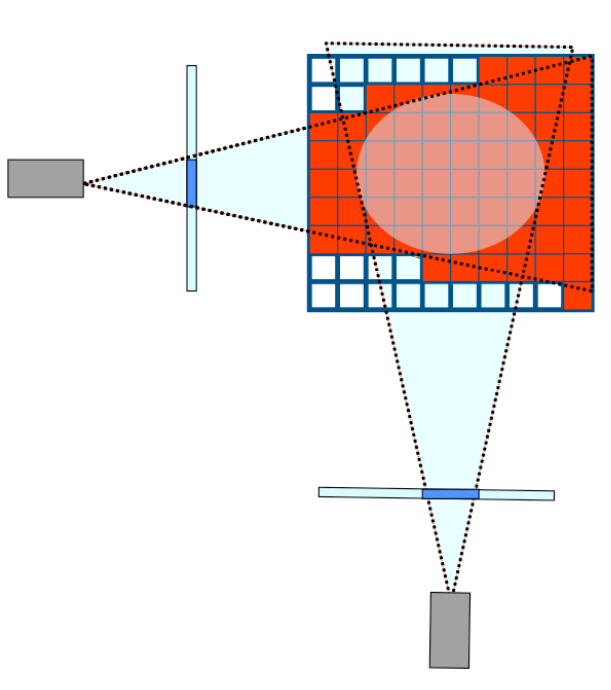
\includegraphics[width = 0.8\textwidth]{figures/space_carving.png}
    \caption{The result of space carving when done on a voxel grid. The region is the reconstructed object after carving from two views, while the shaded part on the inside is the actual object. Notice that the reconstruction is always conservative.}
    \label{fig:space_carving}
\end{figure}

In practice, we first begin by defining a working volume that we know the object is contained within. For example, if our cameras encircle the object, then we can simply say that the working volume is the entire interior of the space enclosed by the cameras. We divide this volume into small units known as \emph{voxels}, defining what is known as a voxel grid. We take each voxel in the voxel grid and project it into each of the views. If the voxel is not contained by the silhouette in a view, then it is discarded. Consequently, at the end of the space carving algorithm, we are left with the voxels that are contained within the visual hull.

Although the space carving method avoids the correspondence problem and is relatively straightforward, it still has many limitations. One limitation of space carving is that it scales linearly with the number of voxels in the grid. As we reduce the size of each voxel, the number of voxels required by the grid increases cubically. Therefore, to get finer reconstruction results in much larger run time. However, some methods such as using octrees can be used mitigate this problem. Related, but simpler methods include doing iterative carvings to reduce the size of the initial voxel grid. 

\begin{figure}[h!]
    \centering
    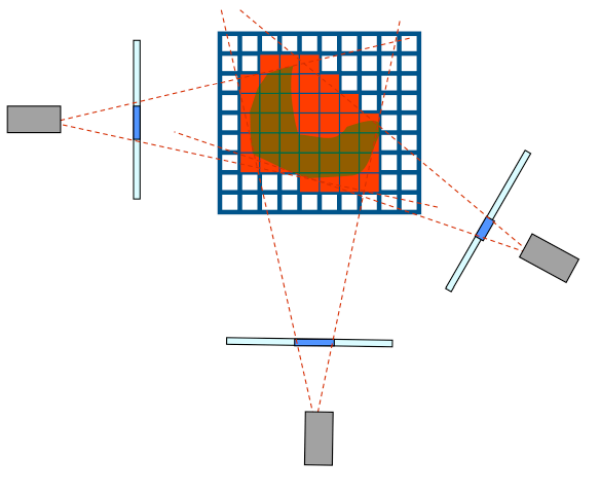
\includegraphics[width = 0.8\textwidth]{figures/concavity.png}
    \caption{Space carving cannot handle some concavities, as demonstrated here, because it cannot carve into that region, as doing so will carve through the object. Note this means that generally the only concavities that space carving can handle are holes through an object. }
    \label{fig:concavity}
\end{figure}

Another limitation is that the efficacy of space carving is dependent on the number of views, the preciseness of the silhouette, and even the shape of the object we are trying to reconstruct. If the number of views is too low, then we end of up with a very loose estimate of the visual hull of the object. As the number of views increases, the more extraneous voxels can be removed by the consistency check. Furthermore, the validity of the consistency check is solely upheld by the fact that we believe that the silhouettes are correct. If the silhouette is too conservative and contains more pixels than necessary, then our carving may not be precise. In a potentially even worse case, the silhouette misses portions of the actual object, resulting in a reconstruction that is overly carved. Finally, a major drawback of space carving is that it is incapable of modeling certain concavities of an object, as shown in Figure~\ref{fig:concavity}.

\subsection{Shadow carving}
To circumvent the concavity problem posed by space carving, we need to look to other forms of consistency checks. One important cue for determining the 3D shape of an object that we can use is the presence of \emph{self-shadows}. Self-shadows are the shadows that an object projects on itself. For the case of concave objects, an object will often cast self-shadows in the concave region. 

\begin{figure}[h!]
    \centering
    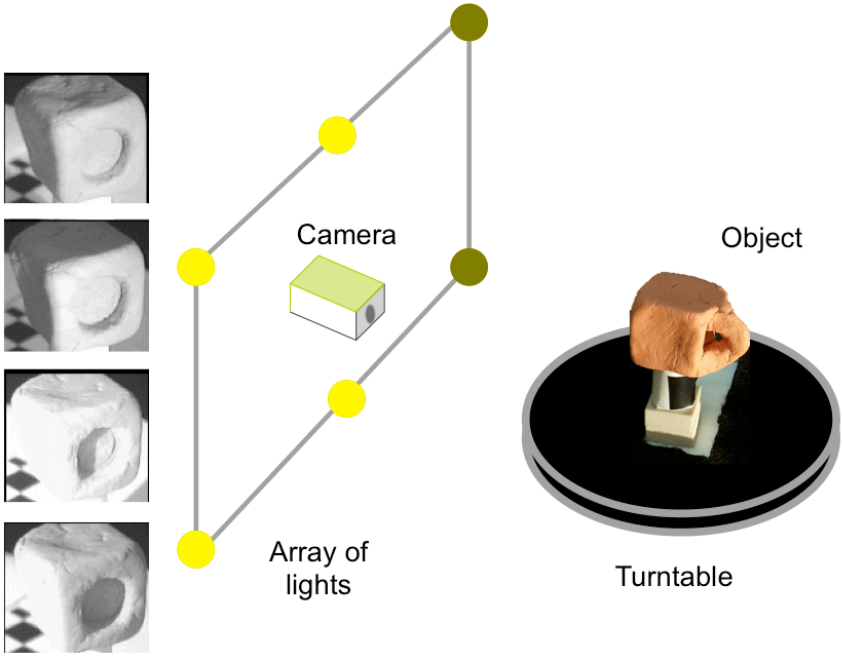
\includegraphics[width = 0.8\textwidth]{figures/shadow_carving.png}
    \caption{The setup of shadow carving, which augments space carving by adding a new consistency check from an array of lights surrounding the camera.}
    \label{fig:shadow_carving}
\end{figure}

\emph{Shadow carving} at its core augments space carving with the idea of using self-shadows to better estimate the concavities. As shown in Figure~\ref{fig:shadow_carving}, the general setup of shadow carving is very similar to space carving. An object is placed in a turntable that is viewed by a calibrated camera. However, there is an array of lights in known positions around the camera whose states can be appropriately turned on and off. These lights will be used to make the object cast self-shadows.

\begin{figure}[h!]
    \centering
    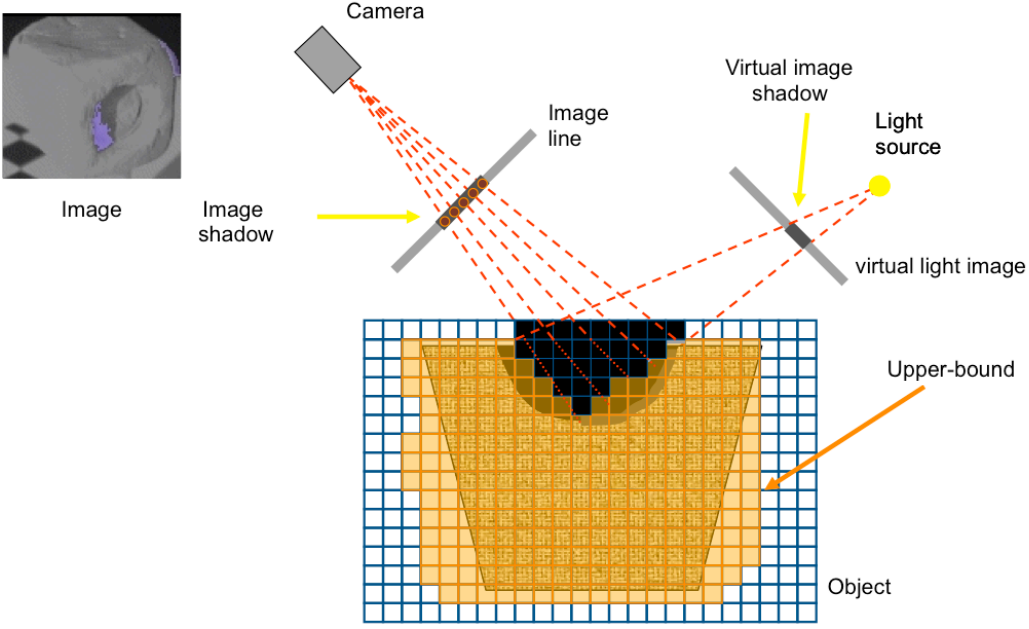
\includegraphics[width = 0.8\textwidth]{figures/shadow_carving_detailed.png}
    \caption{Shadow carving relies on a new consistency check that removes voxels that are in the self-shadow visual cone of the camera and the visual cone of the light.}
    \label{fig:shadow_carving_detailed}
\end{figure}

As shown in Figure~\ref{fig:shadow_carving_detailed}, the shadow carving process begins with an initial voxel grid, which is trimmed down by using the same approach as in space carving. However, in each view, we can turn on and off each light in the array surrounding the camera. Each light will produce a different self-shadow on the object. Upon identifying the shadow in the image plane, we can then find the voxels on the surface of our trimmed voxel grid that are in the visual cone of the shadow. These surface voxels allow us to then make a new visual cone with the image source. We then leverage the useful fact that a voxel that is part of both visual cones cannot be part of the object to eliminate voxels in the concavity. 

Like space carving, the runtime of shadow carving is dependent on the resolution of the voxel grid. The runtime scales cubically with the resolution of the voxel grid. However, if there are $N$ lights, then shadow carving takes approximately $N+1$ times longer than space carving, as each voxel needs to be projected into the camera and each of the $N$ lights can be turned on and off.

In summary, shadow carving always produces a conservative volume estimate that better reconstructs 3D shapes with concavities. The quality of the results depends on both the number of views and the number of light sources. Some disadvantages of this approach are that it cannot handle cases where the object contains reflective or low albedo regions. This is because shadows cannot be detected accurately in such conditions.

\subsection{Voxel coloring}
The last technique we cover in volumetric stereo is \emph{voxel coloring}, which uses color consistency instead of contour consistency in space carving.

\begin{figure}[h!]
    \centering
    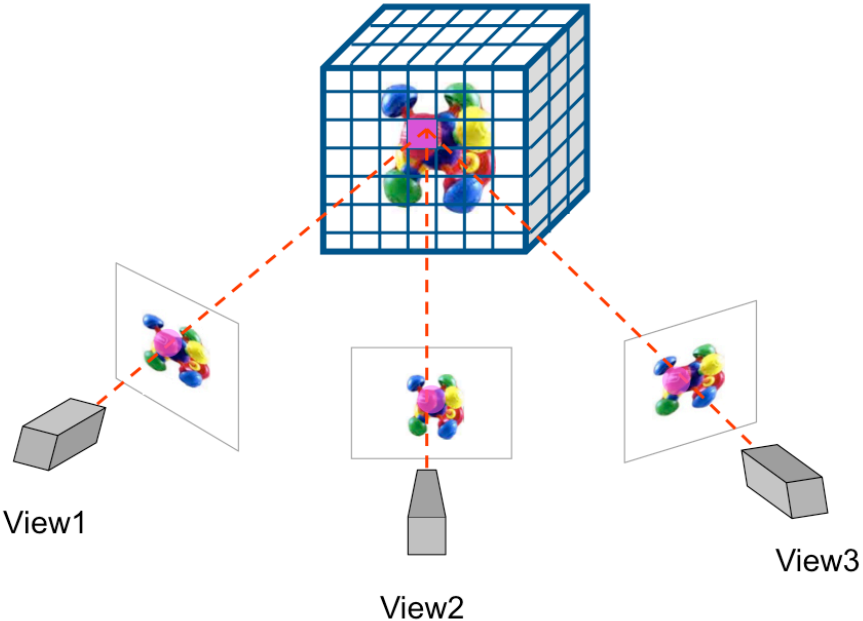
\includegraphics[width = 0.8\textwidth]{figures/voxel_coloring.png}
    \caption{The setup of voxel coloring, which makes a consistency check of the color of all projections of a voxel.}
    \label{fig:voxel_coloring}
\end{figure}

As illustrated in Figure~\ref{fig:voxel_coloring}, suppose that we are given images from multiple views of an object that we want to reconstruct. For each voxel, we look at its corresponding projections in each of the images and compare the color of each of these projections. If the colors of these projections sufficiently match, then we mark the voxel as part of the object. One benefit of voxel coloring not present in space carving is that color associated with the projections can be transferred to the voxel, giving a colored reconstruction.

Overall, there are many methods that one could use for the color consistency check. One example would be to set a threshold between the color similarity between the projections. However, there exists a critical assumption for any color consistency check used: the object being reconstructed must be \emph{Lambertian}, which means that the perceived luminance of any part of the object does not change with viewpoint location or pose. For non-Lambertian objects, such as those made of highly reflective material, it is easy to conceive that the color consistency check would fail on voxels that are actually part of the object.

\begin{figure}[h!]
    \centering
    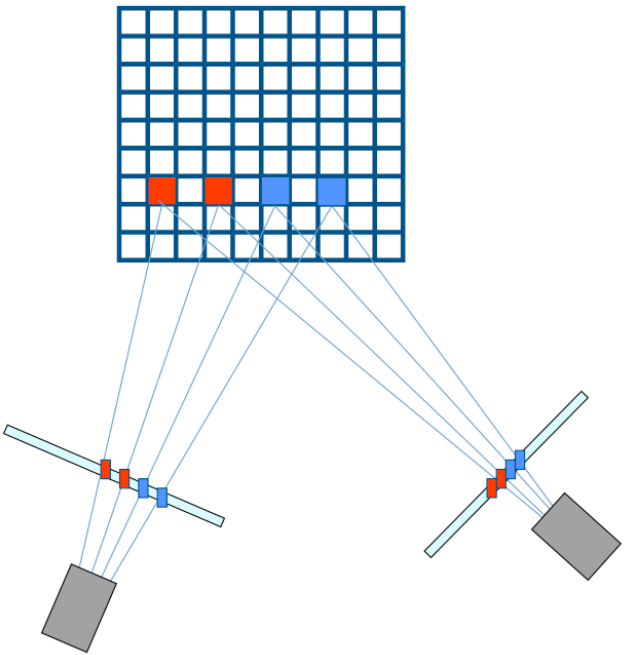
\includegraphics[width = 0.4\textwidth]{figures/ambiguity1.png}
    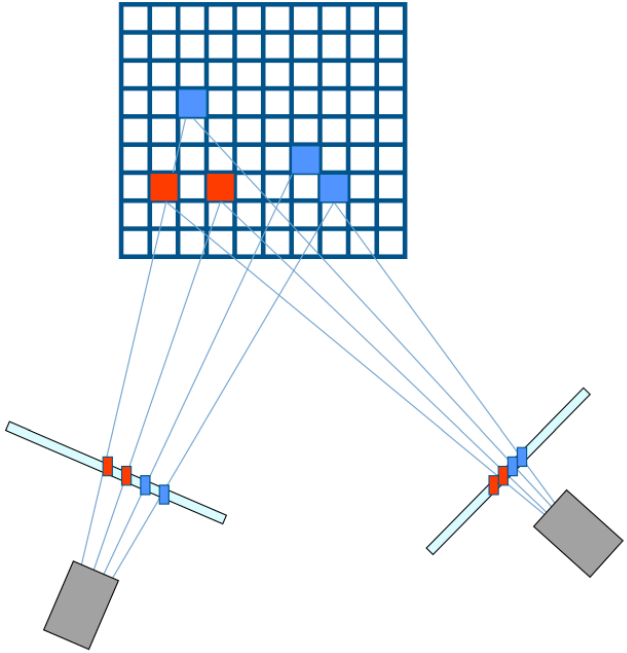
\includegraphics[width = 0.4\textwidth]{figures/ambiguity2.png}
    \caption{An example of an ambiguous case of vanilla voxel coloring.}
    \label{fig:ambiguity}
\end{figure}

One drawback of vanilla voxel coloring is that it produces a solution that is not necessarily unique, as shown in Figure~\ref{fig:ambiguity}. Finding the true, unique solution complicates the problem of reconstruction by voxel coloring. It is possible to remove the ambiguity in the reconstruction by introducing a visibility constraint on the voxel, which requires that the voxels be traversed in a particular order. 

In particular, we want to traverse the voxels layer by layer, starting with voxels closer to the cameras and then progress to further away voxels. When using this order, we perform the color consistency check. Then, we check if the voxel is viewable by at least two of the cameras, which constructs our visibility constraint. If the voxel was not viewable by at least two cameras, then it must be occluded and thus not part of the object. Notice that our order of processing the closer voxels allows us to make sure that we keep the voxels that can occlude later processed voxels to enforce this visibility constraint. 

To conclude, voxel coloring has the advantage of simultaneously capturing the shape and texture of an object. Some of the drawbacks include that the object is assumed to be Lambertian and that the cameras cannot be in certain locations, as the voxels need to be processed in a certain order due to the visibility constraint.
\end{document}
